%-----------------------------------------------------------------------------
%
%               Template for sigplanconf LaTeX Class
%
% Name:         sigplanconf-template.tex
%
% Purpose:      A template for sigplanconf.cls, which is a LaTeX 2e class
%               file for SIGPLAN conference proceedings.
%
% Guide:        Refer to "Author's Guide to the ACM SIGPLAN Class,"
%               sigplanconf-guide.pdf
%
% Author:       Paul C. Anagnostopoulos
%               Windfall Software
%               978 371-2316
%               paul@windfall.com
%
% Created:      15 February 2005
%
%-----------------------------------------------------------------------------


\documentclass[10pt,reprint]{socc14}

\usepackage{amsmath}
\usepackage{mathptmx}
\usepackage{graphicx}
\usepackage{epsfig}

\begin{document}

\special{papersize=8.5in,11in}
\setlength{\pdfpageheight}{\paperheight}
\setlength{\pdfpagewidth}{\paperwidth}

\conferenceinfo{Submission to SoCC '15}{August, 2015, Waikoloa, HI, USA} 
\copyrightyear{2015} 
\copyrightdata{978-1-nnnn-nnnn-n/yy/mm} 
\doi{nnnnnnn.nnnnnnn}

% Uncomment one of the following two, if you are not going for the 
% traditional copyright transfer agreement.

%\exclusivelicense                % ACM gets exclusive license to publish, 
                                  % you retain copyright

%\permissiontopublish             % ACM gets nonexclusive license to publish
                                  % (paid open-access papers, 
                                  % short abstracts)

%\titlebanner{banner above paper title}        % These are ignored unless
%\preprintfooter{short description of paper}   % 'preprint' option specified.

\title{SciPaaS: A Scientific Execution Platform for the Cloud}
%\subtitle{Subtitle text, if any}

\authorinfo{Wesley Brewer}
           {Fluid Physics International}
           {wes@fluidphysics.com}
\authorinfo{Will Scott}
           {Univ. of Washington}
           {Department of Computer Science}
           {wrs@cs.washington.edu}
\authorinfo{John Sanford}
           {Cornell University}
           {Department of Hort. Science}
           {jcs21@cornell.edu}

\maketitle

\begin{abstract}
SciPaaS is a prototype development of an execution platform/middleware designed to make it easy for scientists to rapidly deploy their scientific applications (apps) to the cloud.  It provides all the necessary infrastructure for running typical IXP (Input-eXecute-Plot) style apps, including: a web interface, post-processing and plotting capabilities, job scheduling, real-time monitoring of running jobs, and even a file/case manager.   In this paper, first the system architecture is described and then is demonstrated on an Amazon EC2 instance for the scientific application Mendel’s Accountant—a forward-time population genetics simulation model.  The implications of the prototype are discussed in terms of ease-of-use and deployment options, especially in cloud environments.
\end{abstract}

\category{C.2.4}{Distributed Systems}{Distributed Applications}

% general terms are not compulsory anymore, 
% you may leave them out
\terms
Science, Cloud, Simulation

\keywords
Platform-as-a-Service (PaaS), rapid application development (RAD), population genetics

\section{Introduction}

Scientific programmers very often invest enormous amounts of time and resources developing sophisticated computer programs for specific technical applications. Many of these programs are both brilliant and elegant, and are potentially of interest to a significant number of users beyond just the developers. Most of these programs do not have a broad enough potential user base to justify custom development of sophisticated, easily exported, plug-in, user-friendly input/output, turnkey systems.  As a consequence, many wonderful programs are used for just a few years, by just a handful of people (the developers and their extended team), and then fall into disuse. The utilization of such programs could be greatly enhanced if only they were easily accessed, configured, and operated.

Unfortunately, most scientific programs have been developed in a way that is not easily distributed, nor easily installed, nor easily configured. To make matters worse, there is usually a serious learning curve in terms of using a program. Lastly, many people who might like to use a given program are not themselves programmers – they may be, for example, biologists.  For a biologist to understand how to use a program, and how to interpret the output, requires an extremely user-friendly user interface.  All these problems combine to create an enormous barrier to full utilization of scientific programs. The learning curve is too long and user pain is too great. The cost of getting started is very often too high, and the benefits are often uncertain. 
While the cloud is a very versatile and powerful resource, most scientists have little knowledge about the cloud, and much less about how to build a Software-as-as-Service (SaaS). In general, web interface tools that require little programming skill have little capability (e.g. blog), while more powerful tools (e.g. a full stack web framework) have much capability, but require more programming skills. As illustrated in Fig. \ref{spectrum}, Karger suggests that domain tools can be developed which provide high power while requiring low complexity \cite{karger14}. In the domain of science, SciPaaS seeks to fill this void.

The concept of SciPaaS is that a scientist could easily create a zip archive of their code containing just the executable and a sample input file, upload it to the cloud, and SciPaaS would manage all the cloud infrastructure for them, including the input interface, job scheduling, plotting, etc.  This allows the scientists to focus on developing software to solve the problem at hand, without having to worry about the added overhead of developing the infrastructure for the execution and interface environment.

We outline here a generic system for the easy packaging, uploading, configuration, and utilization of any technical program that would otherwise not find application beyond the development team. We illustrate the utility of this system using the technical program called Mendel’s Accountant – an advanced numerical simulation of the dynamics of mutation accumulation within biological populations that are undergoing natural selection \cite{sanford07}.

\begin{figure}[t]
\centering
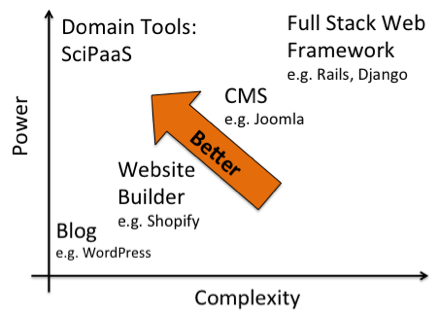
\includegraphics[natwidth=440,natheight=314]{figs/spectrum.png}
%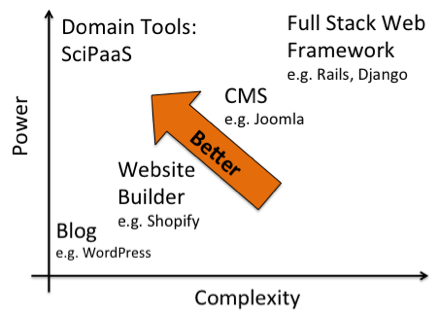
\includegraphics[trim=100 -100 440 314,clip,natwidth=440,natheight=314]{figs/spectrum.png}
%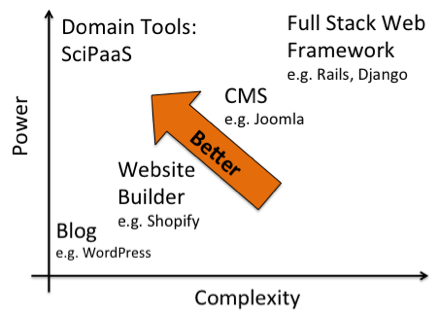
\includegraphics[trim=left bottom right top, clip]{figs/spectrum.png}
%\epsfig{figure=figs/spectrum.eps,width=3in}
\caption{Spectrum of web interface capabilities \cite{karger14} \label{spectrum}}
\end{figure}

\section{Background}

A thorough overview of developments of web-based simulations (WBS) and tools has been well documented by Byrne et al. \cite{byrne10}.  In this review, the authors emphasize the development of web simulations in light of more recent prominence of technologies such as: Web 2.0 (including cloud computing), service-oriented architectures (SOA), and the Semantic Web.  They mention numerous different types of communications protocols such as using WSDL (web-service definition language) or Java remote method invocation (RMI).

 More recently, there has been a number of software packages developed over the past few years to address the need of being able to run scientific applications on a computer cluster. Wu et al. \cite{wu10} developed a scientific application framework based on OpenSocial gadgets.  Krishnan et al. \cite{krishnan10} developed Opal2, a toolkit basically which can be used to wrap scientific applications and expose them as web services.   Opal2 also provides plugin integration with EC2 and Hadoop.  Opal2 provides much of the backend infrastructure for running applications, but relies on other software such as Kepler for pre-processing, and other codes for post-processing.  
During the last couple years, there some new architectures and design methodologies have been proposed for cloud-based simulations.  Hu et al. \cite{hu13} compare four different modern methodologies (simulation model portability [SMP], MyExperiment, NanoHub, and RunMyCode), which promote reuse among common components in cloud-based simulation.  

The concept of NanoHub, a scientific hub for web-based simulation for nanotechnology, is based on the HUBZero open source software platform, which uses a typical LAMP-stack (in this case Linux, Apache, MySQL, PHP) approach for the website and content-management system (CMS), while using a Java-based toolkit called Rappture (Rapid Application Infrastructure) to enable legacy scientific applications to run on the web \cite{mclennan10}.

Di Pierro \cite{dipierro11} developed a python-based web framework called web2py.  He uses web2py to show a sample scientific computing application in which stores DNA strings and searches for similarities.  One of the powerful features of web2py is that it uses in data access layer (DAL) such that many different types of database systems can be supported, including both relational and non-relational models.  In fact, SciPaaS uses a version of the DAL from web2py called Gluino.

Liu et al. \cite{liu12} provide a detailed architecture for Cloud-based Simulation (csim), where they define three key cloud services related to simulation in the cloud: Modeling as a Service (MaaS), Execution as a Service (EaaS), and Analysis as a Service (AaaS).  

Then they discuss more about more efficient ways of scheduling parallel and distributed applications (PADS) and then present four PADS job scheduling algorithms. 
Although other methods exist for creating scientific hubs, they typically require much programming, knowledge and time to setup.  To the authors knowledge there are still no available frameworks or middleware solutions that are dedicated to supporting scientific applications in such a way that: (1) a user can easily upload their program to the cloud, (2) have a user-friendly interface automatically generated for them to run, and (3) provide the infrastructure for all common tasks such as job scheduling, plotting, file/case management, etc.

\section{System Architecture}

The concept for SciPaaS resulted from identifying the common reusable components in many IXP (Input-eXecute-Plot) style software systems as shown in Fig. \ref{ixp}, such as:

\begin{figure}[t]
\centering
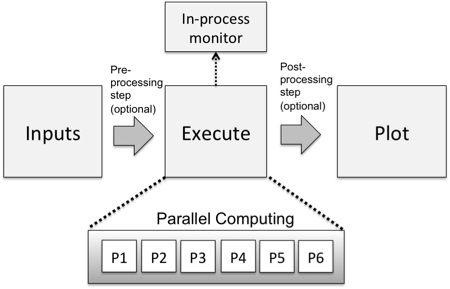
\includegraphics[natwidth=450,natheight=289]{figs/ixp.png}
\caption{Many scientific applications fall under an Input-eXecute-Plot (IXP) design pattern. \label{ixp}}
\end{figure}

\begin{itemize}
\item Interface design
\item User authentication
\item Job scheduling
\item Plotting system
\item In-process monitoring
\item Management of parallel jobs
\end{itemize}

Traditionally, developers would use third-party software was used to handle each of these components.  The problem with using third-party software was that it made it very difficult to setup the environment on the machine to run the simulation.  For example, often OpenPBS (currently rebranded as “Torque”) is implemented as a job scheduler.  This one software alone can take quite some time to setup, is non-trivial to manage, and is overkill for managing software running in a single computer node.

By considering a number of similar type software, the following design goals were identified.  SciPaaS should:

\begin{itemize}
\item Automatically build a web interface
\item Manage job execution, scheduling, and monitoring
\item Monitor simulation as it is running
\item Provide a plotting library interface
\item Handle multiple users
\item Provide a file/case manager
\item Easily be deployed onto Amazon EC2, Google App Engine (GAE), Google Compute Engine (GCE), or RedHat OpenShift.
\end{itemize}

To meet these design goals, the following approach was used:

\begin{itemize}
\item Use a MVT python-based web framework
\item Use a simple DB-based scheduler
\item Build to support standard scientific application design patterns
\end{itemize}

After considering a number of alternative languages, such as Java and Ruby, Python was chosen for three reasons: (1) it has one of the largest scientific computing communities, which includes scientific computing libraries such as SciPy (scipy.org), NumPy (numpy.org), and Matplotlib (matplotlib.org), (2) there are numerous open-source python-based web application frameworks available, and (3) because many of the cloud PaaS providers support Python-based applications (e.g. Google App Engine and Heroku). 

\section{Discussion}

In this section we describe each of the main components of the SciPaaS platform.

\subsection{Upload app to cloud}

A zipfile containing a default input file and binary of the application is uploaded to SciPaaS.  The upload process unzips the file to the appropriate locations, reads the default input deck, and then creates an HTML template file views folder named the same as the application.  The next section explains how the interface is generated from the input deck.

\subsection{Auto-interface generation}

SciPaaS can be used to automatically generate an HTML interface given an input deck as shown in Fig. 3.  Currently three different types of standard input deck formats are supported: (1) namelist input decks which are typically used in Fortran 90 scientific applications, and (2) INI format which is a standard configuration file typically used in Windows applications, and (3) xml format commonly used in Java applications among others.

While the namelist reader/writer had to be custom written for SciPaaS, the INI reader/writer makes use of Python’s built-in ConfigParser module.  In Fig. \ref{interface}, we show a portion of the Mendel input deck, and then the HTML template file that SciPaaS automatically generates.

Finally, there are some applications that will require a customized reader/writer.  In these cases, the user can write their own plugin module with reader/writer methods for reading and writing their own customized input deck.

\begin{figure}[t]
\centering
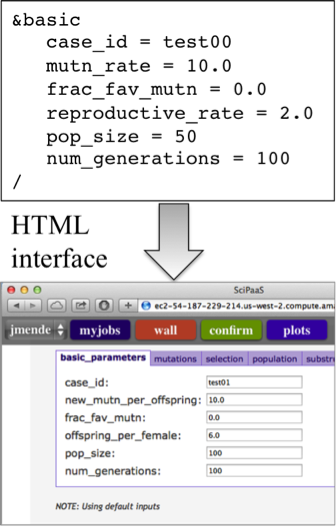
\includegraphics[natwidth=336,natheight=527]{figs/interface.png}
\caption{SciPaaS automatically converts input file to HTML form. \label{interface}}
\end{figure}

\subsection{Web Framework}

The core of SciPaaS is based on a micro-web framework called Bottle (bottlepy.org).  This was chosen over a full stack framework to keep the design simple with no external dependencies.  Bottle uses a model-view-template (MVT) architecture as shown in Fig. \ref{arch}, combined with a separate scheduler, and data access layer, which are later discussed.  The main purpose of the web framework is to map URL routes to Python methods, but it also provides a simple, yet powerful templating system.  While Bottle is not a full stack framework, it is easily extended via many third-party plugins to provide almost any feature that a full stack support, e.g. object-relational mapping (ORM), session management, flash messages, etc.

\begin{figure}[t]
\centering
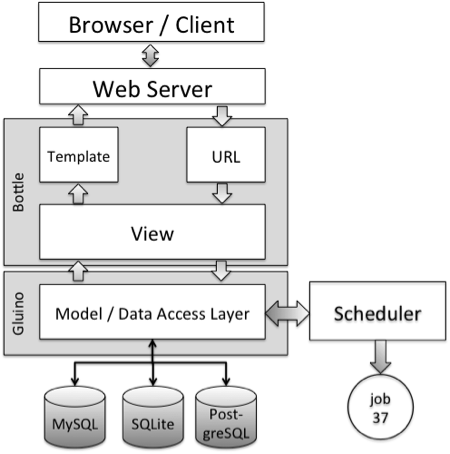
\includegraphics[natwidth=450,natheight=454]{figs/arch.png}
\caption{SciPaaS architecture. \label{arch}}
\end{figure}

\subsection{Database}

SciPaaS stores all information about users, apps, jobs, and plots in a database. Gluino, a data access layer (DAL) ported from the web2py web framework was implemented so that many different types of databases could be supported, including: SQLite, PostgreSQL, MySQL, Oracle, Google, and many others \cite{web2py}.

The database manages information about currently installed applications, users, and also information about plotting.  Fig. \ref{arch} shows the general system architecture of the SciPaaS web application framework. Basically the model represents the interface to the database, and the views are essentially HTML templates rendered by Bottle’s template method.

\subsection{Executing the Simulation Engine}

There are several possible ways to spawn the simulation engine from within Python.  One option is to use the \texttt{subprocess} module, which supports either a call method or a pipe.  Another method for spawning the engine is simply to use the system call from the OS module.  The important point is that the job must be launched in the background so that SciPaaS can continue to handle requests.  The way this is handled is by spawning a new thread for every new job that is submitted. The standard output stdout of the simulation is redirected to the file appname.out (e.g. mendel.out in the current example).

\subsection{Plotting the Data}

SciPaas offers two possibilities for plotting: (1) using a jQuery library called Flot, and also (2) using the Matplotlib library to generate static PNG images. Flot is described as “a pure JavaScript plotting library for jQuery, with a focus on simple usage, attractive looks and interactive features”  (flotcharts.org).  The advantage of using a JavaScript/jQuery library is that all the plotting work is offloaded onto the client, rather than putting the burden on the server, and also the user can dynamically interact with the plot (e.g. zooming).  The disadvantage of using Flot is that it has limited support for scientific plots such as contour.  On the other hand, Matplotlib was specifically designed for scientific plotting, and supports many different chart types, including color contours.  The primary disadvantage of using Matplotlib is that it requires installing about six additional third-party packages, whereas Flot does not require any additional software to be installed.

\subsection{Case Management}

Each simulation run is assigned a universal unique identifier (UUID) using Python’s built-in uuid module.  The files and output generated from each run are each stored in their own folder in the relative path user\_data/appname/caseid (e.g. joe/mendel/ c13dxg).

\subsection{Monitoring the Simulation}

Once the simulation has been launched, SciPaaS automatically redirects to the monitor view.  The monitor view is essentially a jQuery AJAX call which repeatedly calls a method called tail, which retrieves the last 40 lines of the output file every second.  

\subsection{Job Scheduler}

A multiprocessing, priority-based FCFS (first-come first-served) scheduler was developed to manage job submissions from the various apps.  The jobs in the queue have three possible states: Q for waiting in queue and R for running or C for completed.  Jobs are submitted to a jobs table in the database, which maintains state information about each job submission. 

Users are assigned priority levels, with 0 having the highest priority.  The admin user has a priority of 0, while regular users are given a priority of 1, and guest users are given a priority of 2. If several jobs are in the queued state, the job with the highest priority (or lowest number) is the first to be selected to run.

The scheduler has a separate polling thread, which repeatedly polls the database every second and starts executing any job that is in the front of the queue, which is in the queued state.  Each job that is launched is run as a separate process using Python’s multiprocessing module.  Administrators can specify the maximum number of processors np that SciPaaS is permitted to use in the config.py file.  When a job finishes, the state is changed from R to C. Fig. \ref{sched} shows a sample output of the job scheduler.

\begin{figure}[t]
\centering
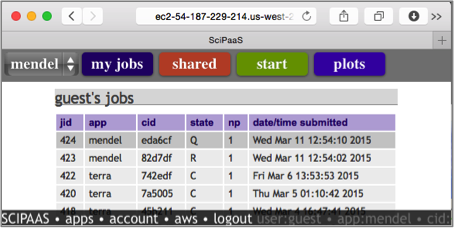
\includegraphics[natwidth=454,natheight=228]{figs/sched.png}
\caption{An example of the built-in job scheduler showing jobs in the queue, running and completed jobs. \label{sched}}
\end{figure}

\subsection{Worker Management}

Integration with the Docker container system is included in SciPaaS in an effort to make deployment of as simple as possible. Docker is a platform and API for application deployment that is supported by most major cloud providers including Google, Microsoft, and Amazon (www.docker.com). When the application finds itself in an environment with a working Docker client, it provides an interface to deploying new workers for scheduled jobs to run on. Additional interface is shown as part of the input screen, allowing the user to choose how many new worker contexts should be used. After use, workers are automatically stopped, making the deployment process simple enough for non-technical users.

\subsection{Example--Mendel's Accountant}

SciPaaS is exemplified using Mendel’s Accountant – a forward-time population genetics simulation program which models genetic change over time.  The software is part of a growing trend of many geneticists turning to computer simulation as a promising means to better understand population genetics \cite{sanford12}. Mendel’s Accountant is more complicated in two aspects: the simulation engine, and the client interface.  

The simulation engine is more complicated because (1) it has more than 60 parameter inputs to the simulation, (2) it is parallelized using the MPI (Message-Passing Interface), (3) generates many output files full of statistical data which needs to be plotted. 

\textit{Pre-processing}. Even though Mendel’s Accountant is a quite complex simulation, since it already supports the standard namelist.input input deck, it can be uploaded and running in the cloud in just a matter of minutes, as shown in Fig. \ref{interface}.

\textit{Processing}.  Fig. \ref{output} shows the console output of Mendel’s Accountant that is auto-updated via AJAX.

\textit{Post-processing}.  Once the run has finished and the data needs to be analyzed, clicking the plot button will given a list of pre-defined plots to plot, or can let the user define new plots.  Data from multiple sources can be attached to each plot. Fig. \ref{neutral} shows bar-plot of the distribution of near-neutral deleterious effects. 

\begin{figure}[t]
\centering
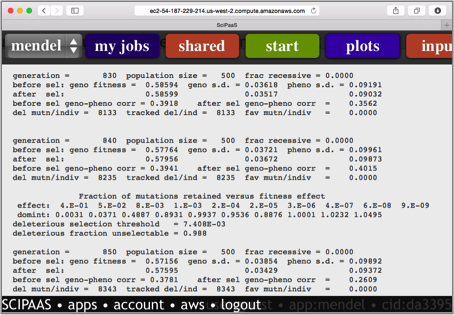
\includegraphics[natwidth=454,natheight=315]{figs/output.png}
\caption{In-process monitoring of Mendel’s Accountant. \label{output}}
\end{figure}

\begin{figure}[t]
\centering
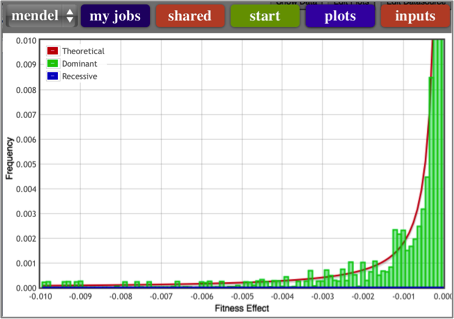
\includegraphics[natwidth=454,natheight=319]{figs/neutral.png}
\caption{Sample output plot of Mendel’s Accountant showing near neutral deleterious effects.\label{neutral}}
\end{figure}

\subsection{Deployment}

For the results for this paper, most of the testing was performed on an Amazon EC2 machine. In the AWS page in SciPaas, the user may store their Amazon instances, and it provides three functions: \textit{start}, \textit{stop}, and \textit{status}. It will also give the user the public DNS name of the machine.  In order to utilize this approach, the user must first setup the various machines they might want to use in the future, which would include installing SciPaaS on each machine.  Then, the user can startup the big machine (e.g. an r3.8xlarge instance which has 32 vCPUs and 244GB of RAM), use it for however long they need, and then download the case files to an inexpensive t1.micro instance, and then shutdown the big, expensive machine. SciPaaS provides a zip button on the my jobs view, which allows the user to compress any case for download either to their home machine, or to another SciPaaS instance.  

\section{Conclusions}

A middleware execution platform called SciPaaS was described and demonstrated with Mendel’s Accountant, a complex forward-time population genetics simulator.   The software will soon be released in the Open Source domain online at https://bitbucket.org/whbrewer/scipaas.

By providing an automatically generated easy-to-use interface, and an easy way to upload and plugin their application to the platform, SciPaaS allows scientists to rapidly deploy their applications to the cloud.

An unintended benefit of this type of platform solution to web-based simulations is that it also encourages developers of scientific simulations towards using standard protocols where appropriate, such as using standardized input formats.

SciPaaS has been tested with a number of scientific software packages, including finite element analysis codes, Hadoop/MapReduce codes for working with big data, in addition to a number of bioinformatics codes.  

Future work should include making SciPaaS more robust by implementing a workflow management system such as Snakemake whereby it could handle more complex software simulation packages that consist of a number of modules.  For example, the Weather Research and Forecasting software (wrf-model.org) includes a number different executables for pre-processing, solving, post-processing, and visualizing large three-dimensional data.  

%\appendix
%\section{Appendix title}
%This is the text of the appendix, if you need one.

\acks

The authors want to acknowledge appreciation for the support graciously provided by FMS Foundation for this project.  Also, thanks to Tichomir Tenev of VMWare for reviewing the manuscript. 
% We recommend abbrvnat bibliography style.

\bibliographystyle{abbrvnat}

% The bibliography should be embedded for final submission.

\begin{thebibliography}{}
\softraggedright

%\bibitem[Smith et~al.(2009)Smith, Jones]{smith02}
%P. Q. Smith, and X. Y. Jones. ...reference text...
\bibitem[]{sanford07} Sanford, J., Baumgardner, J., Brewer, W., Gibson, P., \& ReMine, W. (2007). Mendel's Accountant: A biologically realistic forward-time population genetics program. Scalable Computing: Practice and Experience, 8(2).
\bibitem[]{karger14} Karger, David. “User Interfaces for Data: the Big Picture”, Lecture in Tackling the Challenges of Big Data online course, MIT Professional Education, https://mitprofessionalx.edx.org, 27 October 2014.
\bibitem[]{byrne10} Byrne, James, Cathal Heavey, and Peter J. Byrne. "A review of Web-based simulation and supporting tools." Simulation modeling practice and theory 18.3 (2010): 253-276.
\bibitem[]{wu10} Wu, W., Uram, T., Wilde, M., Herald, M., and Papka, M. “A Web 2.0-Based Scientific Application Framework”, IEEE 2010.
\bibitem[]{krishnan10} Krishnan, S., Clementi, L., Ren, J., Papadopoulos, P., and Li, W.  Design and Evaluation of Opal2: A Tookit for Scientific Software as a Service. 2010
\bibitem[]{hu13} Hu, C., Xu, C., Fan, G., Li, H., Song, D. “A Simulation Model Design Method for Cloud-Based Simulation Environment.  Advances in Mechanical Engineering, Article 932684 (2013).
\bibitem[]{mclennan10} McLennan, M.; Kennell, R., "HUBzero: A Platform for Dissemination and Collaboration in Computational Science and Engineering," Computing in Science and Engineering, 12(2):48-52 (2010).
\bibitem[]{dipierro11} Di Pierro, Massimo, “web2py for Scientific Applications.” Computing in Science \& Engineering 13.2 (2011): 64-69.
\bibitem[]{liu12} Liu, X., Qiu, X., Chen, B., Huang, K. “Cloud-based Simulation: the State-of-the-art Computer Simulation Paradigm”, 2012 ACM/IEEE/SCS 26th Workshop on Principles of Advanced and Distributed Simulation (2012).
\bibitem[]{web2py} Di Pierro, Massimo, web2py Complete Reference Manual (6th edition), http://www.web2py.com/ books/default/chapter/29/06/the-database-abstraction-layer.
\bibitem[]{sanford12} John C. Sanford and Chase W. Nelson (2012). The Next Step in Understanding Population Dynamics: Comprehensive Numerical Simulation, Studies in Population Genetics, Dr. M. Carmen  Fusté (Ed.), ISBN: 978-953-51-0588-6, InTech, DOI: 10.5772/34047.

\end{thebibliography}


\end{document}
